% ============================================================================
% Глава 4: Архитектура на Coroute
% ============================================================================
\section{Архитектура на Coroute}

След като разгледахме теоретичните основи в предходната глава, сега ще представим конкретната архитектура на библиотеката Coroute. Тази глава описва модулната структура на библиотеката, жизнения цикъл на HTTP заявките, корутинния модел на изпълнение, middleware системата и платформено-независимия I/O слой.

Архитектурата на Coroute е проектирана с няколко ключови принципа. Първо, \textbf{модулност} -- всеки компонент има ясно дефинирана отговорност и може да се използва независимо. Второ, \textbf{разширяемост} -- новите протоколи и функционалности могат да се добавят без промяна на съществуващия код. Трето, \textbf{ефективност} -- архитектурата минимизира копирането на данни и системните извиквания. Четвърто, \textbf{безопасност} -- типовата система на C++ се използва за предотвратяване на грешки по време на компилация.

\subsection{Обща архитектура и модулна структура}

Coroute е организиран в йерархия от модули, всеки от които отговаря за определен аспект на функционалността. Тази организация улеснява разбирането на кода, тестването и поддръжката.

Модулът \textbf{core/} съдържа основните компоненти на библиотеката. Класът \texttt{App} е централната точка за конфигуриране и стартиране на сървъра. \texttt{Router} управлява маршрутизирането на заявките към съответните handlers. Класовете \texttt{Request} и \texttt{Response} представляват HTTP заявки и отговори с удобен API за достъп до хедъри, тяло и параметри.

Модулът \textbf{coro/} предоставя корутинната инфраструктура. Типът \texttt{Task<T>} е основният тип за асинхронни операции. \texttt{CancellationToken} позволява кооперативно прекратяване на дълготрайни операции. Тук се намират и различните awaiter типове за интеграция с I/O операциите.

Модулът \textbf{net/} съдържа мрежовия слой. \texttt{IoContext} е абстракция над платформено-специфичните I/O механизми. \texttt{Connection} представлява TCP връзка с методи за асинхронно четене и писане. Тук се намират и имплементациите за TLS и WebSocket.

Модулът \textbf{http2/} съдържа пълната HTTP/2 имплементация. \texttt{Http2Connection} управлява HTTP/2 връзка с множество потоци. HPACK encoder/decoder се грижи за компресията на хедъри. Frame parser/serializer обработва бинарните HTTP/2 фреймове.

Модулът \textbf{util/} съдържа помощни функции и типове. \texttt{expected<T, E>} е тип за представяне на резултат или грешка (подобен на \texttt{std::expected} от C++23). \texttt{FromString<T>} е trait за конвертиране на низове към типове. Тук се намират и функциите за zero-copy file transfer.

\begin{figure}[H]
\centering
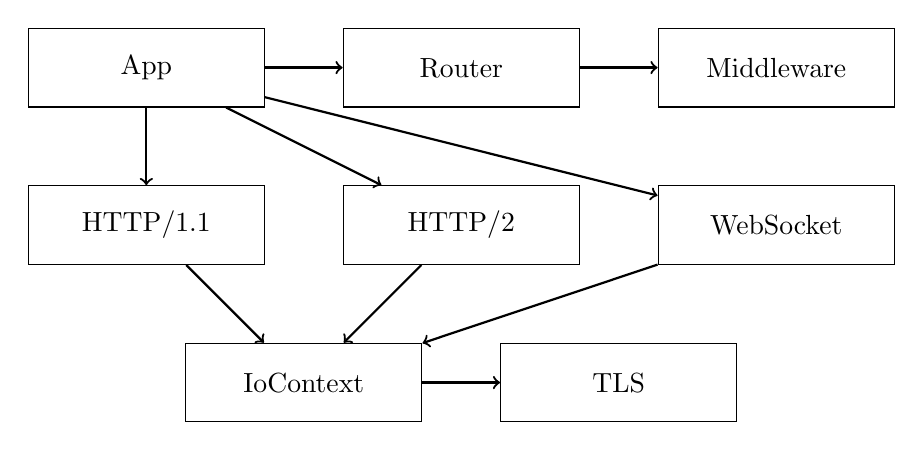
\begin{tikzpicture}[
    box/.style={rectangle, draw, minimum width=3cm, minimum height=1cm, align=center},
    arrow/.style={->, thick}
]
    % Application layer
    \node[box] (app) at (0, 4) {App};
    \node[box] (router) at (4, 4) {Router};
    \node[box] (middleware) at (8, 4) {Middleware};
    
    % Protocol layer
    \node[box] (http11) at (0, 2) {HTTP/1.1};
    \node[box] (http2) at (4, 2) {HTTP/2};
    \node[box] (websocket) at (8, 2) {WebSocket};
    
    % Network layer
    \node[box] (iocontext) at (2, 0) {IoContext};
    \node[box] (tls) at (6, 0) {TLS};
    
    % Arrows
    \draw[arrow] (app) -- (router);
    \draw[arrow] (router) -- (middleware);
    \draw[arrow] (app) -- (http11);
    \draw[arrow] (app) -- (http2);
    \draw[arrow] (app) -- (websocket);
    \draw[arrow] (http11) -- (iocontext);
    \draw[arrow] (http2) -- (iocontext);
    \draw[arrow] (websocket) -- (iocontext);
    \draw[arrow] (iocontext) -- (tls);
\end{tikzpicture}
\caption{Модулна архитектура на Coroute}
\label{fig:architecture}
\end{figure}

\subsection{Жизнен цикъл на HTTP заявка}

Разбирането на жизнения цикъл на HTTP заявката е ключово за ефективното използване на Coroute. Всяка заявка преминава през поредица от етапи, като всеки етап се изпълнява асинхронно чрез корутини.

Първият етап е \textbf{Accept}. IoContext наблюдава listening socket-а за входящи TCP връзки. Когато клиент се свърже, се създава нов \texttt{Connection} обект и се стартира корутина за обработка на връзката. Тази корутина работи в режим ``detached'' -- тя се самоуправлява и се унищожава автоматично при завършване.

Вторият етап е \textbf{TLS Handshake}, който е опционален и се изпълнява само ако сървърът е конфигуриран за HTTPS. По време на handshake се установява криптирана връзка и се верифицира сертификатът на сървъра. TLS handshake също е асинхронен -- корутината спира докато чака завършване на криптографските операции.

Третият етап е \textbf{ALPN Negotiation}, който се случва като част от TLS handshake. Клиентът и сървърът се договарят за протокола -- HTTP/2 (``h2'') или HTTP/1.1 (``http/1.1''). Ако клиентът поддържа HTTP/2 и сървърът е конфигуриран за него, се избира HTTP/2. В противен случай се използва HTTP/1.1.

Четвъртият етап е \textbf{Parse}. Сървърът чете данни от връзката и парсва HTTP заявката. При HTTP/1.1 това включва парсване на request line, хедъри и тяло. При HTTP/2 се декодират бинарни фреймове и HPACK-компресирани хедъри.

Петият етап е \textbf{Route}. DFA matcher-ът съпоставя URL-а на заявката с регистрираните маршрути. Ако има съвпадение, се извличат параметрите от URL-а. Ако няма съвпадение, се връща 404 Not Found.

Шестият етап е \textbf{Middleware}. Заявката преминава през веригата от middleware компоненти. Всеки middleware може да модифицира заявката, да върне отговор директно, или да предаде контрола на следващия middleware.

Седмият етап е \textbf{Handler}. Потребителският handler се извиква с заявката и параметрите. Handler-ът е корутина, която може да извършва асинхронни операции като заявки към база данни или външни API-та.

Осмият етап е \textbf{Response}. Отговорът се сериализира и изпраща към клиента. При HTTP/1.1 това е текстов формат. При HTTP/2 отговорът се разбива на фреймове и хедърите се компресират с HPACK.

Фигура \ref{fig:request-lifecycle} илюстрира пълния жизнен цикъл на HTTP заявка.

\begin{figure}[H]
\centering
\begin{tikzpicture}[
    box/.style={draw, thick, rounded corners, minimum width=2cm, minimum height=0.7cm, font=\small},
    arrow/.style={->, thick, >=stealth},
    scale=0.85
]
    % Main flow
    \node[box, fill=blue!20] (accept) at (0, 0) {Accept};
    \node[box, fill=yellow!20] (tls) at (3, 0) {TLS};
    \node[box, fill=yellow!20] (alpn) at (6, 0) {ALPN};
    \node[box, fill=green!20] (parse) at (9, 0) {Parse};
    \node[box, fill=orange!20] (route) at (12, 0) {Route};
    
    \node[box, fill=purple!20] (mw) at (12, -3) {Middleware};
    \node[box, fill=red!20] (handler) at (9, -3) {Handler};
    \node[box, fill=cyan!20] (response) at (6, -3) {Response};
    \node[box, fill=gray!20] (send) at (3, -3) {Send};
    
    % Arrows
    \draw[arrow] (accept) -- (tls);
    \draw[arrow] (tls) -- (alpn);
    \draw[arrow] (alpn) -- (parse);
    \draw[arrow] (parse) -- (route);
    \draw[arrow] (route) -- (mw);
    \draw[arrow] (mw) -- (handler);
    \draw[arrow] (handler) -- (response);
    \draw[arrow] (response) -- (send);
    
    % Keep-alive loop
    \draw[arrow, dashed, blue] (send.north east) to[out=90, in=-90] node[pos=0.5, below, font=\tiny] {Keep-alive} (parse.south west);
    
    % Optional TLS indicator
    \node[font=\tiny, gray] at (4.5, 0.7) {HTTPS only};
    \draw[gray, dashed] (2, 0.5) -- (7,0.5);
    
    % Annotations
    \node[font=\tiny, align=center] at (0, -0.9) {TCP\\връзка};
    \node[font=\tiny, align=center] at (3, -0.9) {Криптиране\\(опционално)};
    \node[font=\tiny, align=center] at (6, -0.9) {Избор на протокол};
    \node[font=\tiny, align=center] at (9, -0.9) {HTTP\\парсване};
    \node[font=\tiny, align=center] at (12, -0.9) {DFA\\маршрут};
    
    % Coroutine indicator
    \draw[decorate, decoration={brace, amplitude=5pt}, thick, green!60!black] 
        (-0.8, 1) -- (12.8, 1) node[midway, above=5pt, font=\tiny] {Всеки етап е co\_await точка};
\end{tikzpicture}
\caption{Жизнен цикъл на HTTP заявка в Coroute}
\label{fig:request-lifecycle}
\end{figure}

Следният код от \texttt{app.cpp} илюстрира основния accept loop:

\begin{lstlisting}[language=C++, basicstyle=\small\ttfamily, caption={Основен accept loop}]
[this]() -> Task<void> {
    while (!cancel_source_.is_cancelled()) {
        auto conn_result = co_await listener_->async_accept();
        if (!conn_result) {
            if (cancel_source_.is_cancelled()) break;
            continue;
        }
        handle_connection(std::move(*conn_result)).start_detached();
    }
}().start_detached();
\end{lstlisting}

Методът \texttt{start\_detached()} стартира корутината в режим ``fire-and-forget'' -- тя се самоунищожава при завършване.

\subsection{Корутинен модел на изпълнение -- Task<T>}

Централен елемент на Coroute е типът \texttt{Task<T>}, който представлява асинхронна операция, връщаща стойност от тип \texttt{T}. Този тип е сърцето на корутинната инфраструктура и определя как корутините се създават, изпълняват и завършват.

\texttt{Task<T>} е проектиран да бъде ``lazy'' -- корутината не започва изпълнение при създаване, а чак когато бъде awaited. Това позволява композиране на корутини без нежелани странични ефекти. Също така, \texttt{Task<T>} поддържа режим ``detached'', при който корутината се самоуправлява и се унищожава автоматично при завършване.

\subsubsection{Promise Type}

Всяка корутина в C++ има асоцииран \texttt{promise\_type}, който контролира нейното поведение. Promise type-ът определя какво се случва при различните етапи от живота на корутината -- създаване, спиране, възобновяване и завършване.

\begin{lstlisting}[language=C++, basicstyle=\small\ttfamily, caption={TaskPromiseBase структура}]
struct TaskPromiseBase {
    std::coroutine_handle<> continuation_ = std::noop_coroutine();
    std::exception_ptr exception_;
    CancellationToken cancel_token_;
    bool detached_ = false;

    std::suspend_always initial_suspend() noexcept { return {}; }
    FinalAwaiter final_suspend() noexcept { return {}; }
    
    void unhandled_exception() noexcept {
        exception_ = std::current_exception();
    }
};
\end{lstlisting}

\textbf{Ключови характеристики:}
\begin{itemize}
    \item \texttt{initial\_suspend()} връща \texttt{suspend\_always} -- корутината е ``lazy'' и не започва изпълнение докато не бъде awaited
    \item \texttt{continuation\_} съхранява handle към извикващата корутина за възобновяване
    \item \texttt{detached\_} флаг указва дали корутината трябва да се самоунищожи
\end{itemize}

\subsubsection{FinalAwaiter}

При завършване на корутината, \texttt{FinalAwaiter} решава какво да се случи:

\begin{lstlisting}[language=C++, basicstyle=\small\ttfamily, caption={FinalAwaiter логика}]
struct FinalAwaiter {
    template<typename Promise>
    std::coroutine_handle<> await_suspend(
        std::coroutine_handle<Promise> h) noexcept {
        auto& promise = h.promise();
        
        // If detached, destroy ourselves
        if (promise.detached_) {
            h.destroy();
            return std::noop_coroutine();
        }
        
        // Resume continuation if exists
        if (promise.continuation_) {
            return promise.continuation_;
        }
        return std::noop_coroutine();
    }
};
\end{lstlisting}

\subsubsection{Awaiter}

Когато една корутина ``await-ва'' \texttt{Task<T>}, се използва следният awaiter:

\begin{lstlisting}[language=C++, basicstyle=\small\ttfamily, caption={Task Awaiter}]
struct Awaiter {
    handle_type handle_;

    bool await_ready() const noexcept {
        return !handle_ || handle_.done();
    }

    std::coroutine_handle<> await_suspend(
        std::coroutine_handle<> continuation) noexcept {
        handle_.promise().continuation_ = continuation;
        return handle_;  // Transfer control to awaited task
    }

    T await_resume() {
        return std::move(handle_.promise()).result();
    }
};
\end{lstlisting}

\subsection{Безопасност на паметта при detached корутини}

Използването на \texttt{start\_detached()} въвежда специфични предизвикателства за управление на паметта. Когато корутина работи в detached режим, тя няма ``собственик'' --- никой не чака нейното завършване и никой не държи reference към нея. Това създава риск от \texttt{use-after-free} грешки, ако корутината достъпва ресурси, които са били унищожени.

\subsubsection{Проблемът}

Разгледайте следния опасен код:

\begin{lstlisting}[language=C++, basicstyle=\small\ttfamily, caption={Опасен pattern с detached корутина}]
void dangerous_example() {
    std::string local_data = "important";
    
    [&local_data]() -> Task<void> {
        co_await async_delay(100ms);
        // DANGER: local_data may be destroyed!
        std::cout << local_data << std::endl;
    }().start_detached();
}  // local_data is destroyed here
\end{lstlisting}

Когато \texttt{dangerous\_example()} завърши, \texttt{local\_data} се унищожава, но detached корутината все още може да работи и да се опита да достъпи унищожената памет.

\subsubsection{Решения в Coroute}

Coroute използва няколко техники за предотвратяване на тези проблеми:

\textbf{1. Move семантика за Connection:}
\begin{lstlisting}[language=C++, basicstyle=\small\ttfamily, caption={Безопасно предаване на ownership}]
handle_connection(std::move(*conn_result)).start_detached();
\end{lstlisting}

Connection обектът се \texttt{move}-ва в корутината, която поема пълната отговорност за неговия живот. Корутината унищожава connection-а при завършване.

\textbf{2. RAII guards за ресурси:}
\begin{lstlisting}[language=C++, basicstyle=\small\ttfamily, caption={RAII pattern за connection lifecycle}]
Task<void> handle_connection(std::unique_ptr<Connection> conn) {
    // conn is owned by this coroutine
    // It will be destroyed when coroutine completes
    
    while (!cancel_token.is_cancelled()) {
        auto data = co_await conn->async_read(...);
        if (!data) break;
        // process...
    }
    
    conn->close();  // Explicit cleanup
}  // conn destroyed here automatically
\end{lstlisting}

\textbf{3. Shared ownership когато е необходимо:}
\begin{lstlisting}[language=C++, basicstyle=\small\ttfamily, caption={Shared ownership за споделени ресурси}]
auto shared_state = std::make_shared<SessionState>();

[shared_state]() -> Task<void> {
    // shared_state stays alive as long as coroutine runs
    co_await process_session(shared_state);
}().start_detached();
\end{lstlisting}

\textbf{4. CancellationToken за кооперативно прекратяване:}

При shutdown, сървърът сигнализира на всички активни корутини да завършат чрез \texttt{CancellationToken}. Това позволява graceful cleanup вместо насилствено прекратяване.

\subsubsection{Правила за безопасност}

При работа с detached корутини в Coroute, следвайте тези правила:
\begin{enumerate}
    \item Никога не capture-вайте локални променливи по reference в detached корутина
    \item Използвайте \texttt{std::move()} за прехвърляне на ownership
    \item За споделени ресурси използвайте \texttt{std::shared\_ptr}
    \item Винаги проверявайте \texttt{CancellationToken} в дълготрайни операции
\end{enumerate}

\subsection{DFA-базирано маршрутизиране}

Coroute използва алгоритъма, описан в „Matching Text from Start to Finish Against Multiple Regular Expressions" \cite{stankov2024regex}, за ефективно маршрутизиране на заявки.

\subsubsection{Регистрация на маршрути}

Маршрутите се регистрират чрез методите \texttt{get()}, \texttt{post()}, и др.:

\begin{lstlisting}[language=C++, basicstyle=\small\ttfamily, caption={Регистрация на маршрути}]
app.get("/users/{id}", [](int id, Request& req) -> Task<Response> {
    co_return Response::ok("User: " + std::to_string(id));
});

app.post("/api/items", [](Request& req) -> Task<Response> {
    auto body = req.body();
    co_return Response::created(body);
});
\end{lstlisting}

\subsubsection{Конвертиране на шаблони}

Шаблоните се конвертират в регулярни изрази:

\begin{lstlisting}[language=C++, basicstyle=\small\ttfamily, caption={Конвертиране на pattern към regex}]
// /users/{id} -> /users/([A-Za-z0-9_.%-]+)
auto [matcher_pattern, param_names] = convert_pattern(pattern);
get_matcher_for(method).add_regex(matcher_pattern, route_id);
\end{lstlisting}

\subsubsection{Съпоставяне с O(N) сложност}

При получаване на заявка, DFA matcher-ът извършва съпоставяне с линейна сложност:

\begin{lstlisting}[language=C++, basicstyle=\small\ttfamily, caption={DFA matching}]
auto& matcher = get_matcher_for(method);
auto matches = matcher.match_with_groups(std::string(path));

if (!matches.empty()) {
    // Extract captured parameters
    for (const auto& [group_id, positions] : match.groups) {
        result.params[group_id] = path.substr(
            positions.first, 
            positions.second - positions.first
        );
    }
}
\end{lstlisting}

\subsection{Middleware верига}

Middleware компонентите се изпълняват последователно, обвивайки крайния handler.

\subsubsection{Дефиниция на Middleware}

\begin{lstlisting}[language=C++, basicstyle=\small\ttfamily, caption={Middleware тип}]
using Next = std::function<Task<Response>(Request&)>;
using Middleware = std::function<Task<Response>(Request&, Next)>;
\end{lstlisting}

\subsubsection{Рекурсивно изпълнение}

Middleware веригата се изпълнява рекурсивно:

\begin{lstlisting}[language=C++, basicstyle=\small\ttfamily, caption={Изпълнение на middleware верига}]
Task<Response> execute_at(size_t idx, Request& req, Handler handler) {
    if (idx >= middleware_.size()) {
        // Base case: call the handler
        co_return co_await handler(req);
    }
    
    // Create next function
    Next next = [this, idx, &handler](Request& r) -> Task<Response> {
        return execute_at(idx + 1, r, handler);
    };
    
    // Call current middleware
    co_return co_await middleware_[idx](req, next);
}
\end{lstlisting}

\subsubsection{Пример за middleware}

\begin{lstlisting}[language=C++, basicstyle=\small\ttfamily, caption={Authentication middleware}]
Middleware auth_middleware() {
    return [](Request& req, Next next) -> Task<Response> {
        auto token = req.header("Authorization");
        if (!token || !validate_token(*token)) {
            co_return Response::unauthorized("Invalid token");
        }
        
        // Continue to next middleware/handler
        co_return co_await next(req);
    };
}
\end{lstlisting}

\subsection{Платформено-независим I/O слой}

Coroute абстрахира платформено-специфичните I/O механизми зад унифициран интерфейс.

\subsubsection{IoContext интерфейс}

\begin{lstlisting}[language=C++, basicstyle=\small\ttfamily, caption={IoContext абстракция}]
class IoContext {
public:
    // Factory - creates platform-appropriate context
    static std::unique_ptr<IoContext> create(size_t thread_count = 1);
    
    virtual void run() = 0;
    virtual void stop() = 0;
};
\end{lstlisting}

\subsubsection{Connection интерфейс}

\begin{lstlisting}[language=C++, basicstyle=\small\ttfamily, caption={Connection абстракция}]
class Connection {
public:
    virtual Task<ReadResult> async_read(void* buffer, size_t len) = 0;
    virtual Task<WriteResult> async_write(const void* data, size_t len) = 0;
    
    // Zero-copy file transfer
    virtual Task<TransmitResult> async_transmit_file(
        FileHandle file, size_t offset, size_t length) = 0;
};
\end{lstlisting}

\subsubsection{Платформени имплементации}

CMake автоматично избира правилната имплементация:

\begin{lstlisting}[basicstyle=\small\ttfamily, caption={Платформен избор в CMakeLists.txt}]
if(coroute_IO_BACKEND STREQUAL "iocp")
    target_sources(coroute PRIVATE src/net/iocp/iocp_context.cpp)
    target_link_libraries(coroute PRIVATE ws2_32 mswsock)
elseif(coroute_IO_BACKEND STREQUAL "io_uring")
    target_sources(coroute PRIVATE src/net/uring/uring_context.cpp)
    target_link_libraries(coroute PRIVATE uring)
elseif(coroute_IO_BACKEND STREQUAL "kqueue")
    target_sources(coroute PRIVATE src/net/kqueue/kqueue_context.cpp)
endif()
\end{lstlisting}

\subsection{Graceful Shutdown}

Coroute поддържа graceful shutdown за безопасно затваряне на сървъра:

\begin{lstlisting}[language=C++, basicstyle=\small\ttfamily, caption={Graceful shutdown}]
void App::shutdown(ShutdownOptions options) {
    // Mark as shutting down
    shutting_down_.store(true, std::memory_order_relaxed);
    
    // Stop accepting new connections
    listener_->close();
    
    // Wait for existing connections to drain
    auto start = std::chrono::steady_clock::now();
    while (active_connections_.load() > 0) {
        if (elapsed >= options.drain_timeout) break;
        std::this_thread::sleep_for(std::chrono::milliseconds(100));
    }
    
    // Force close if configured
    if (options.force_close_after_timeout) {
        cancel_source_.cancel();
    }
    
    io_ctx_->stop();
}
\end{lstlisting}
